\chapter{Especificación del diseño}\label{chap:design}

\section{Visión general}

Este capítulo tiene como objetivo describir la labor de diseño realizada para desarrollar el proyecto, así como las herramientas que han sido necesarias para su realización. En el siguiente listado se describen los aspectos de diseño que se van a explicar en este capítulo:

\begin{itemize}
	\item \textbf{Diseño de la arquitectura}: descripción del diseño elegido para la arquitectura.
	\item \textbf{Diseño del ``mapeo'' la \acrlong{bd}}: descripción del diseño elegido para el ``mapeo'' de la \acrshort{bd}.
	\item \textbf{Diseño de la aplicación web}: descripción del diseño de la aplicación web.

\end{itemize}

\section{Herramientas utilizadas}

Las herramientas que se han utilizado a la hora de diseñar el proyecto son:

\subsection{Django-extensions, Graph models}

Graph Models es una herramienta para la generación de grafos del modelo relacional a partir de los ficheros \textit{model.py} donde se especifican las clases que conforman el diseño modelo relacional de la aplicación web. Entre algunas de sus características, permite especificar el nombre de varias aplicaciones para combinarlas en un único modelo, incluir herencias, la exclusión de modelos o columnas y modificar la plantilla con la que renderizar el grafo.

Para este proyecto, solo se han usado sus capacidades para renderizar los siguientes grafos, sin los cuales no hubiera sido capaz de entender el modelo relacional de \acrshort{labman} y hacer uso de las tablas necesarias para modificar la capa de datos del servidor MOAI y el filtrado de la búsqueda avanzada de proyectos y publicaciones:

\begin{itemize}
	\item Diagrama del modelo relacional completo, compuesto por todas las entidades de \acrshort{labman}.
	\item Diagrama del modelo relacional de la entidad publicaciones.
	\item Diagrama del modelo relacional de la entidad proyectos.
	\item Diagrama del modelo relacional para el sistema de ``logs'' de Django.
\end{itemize}

\section{Diseño de la arquitectura}

La arquitectura del servidor \acrshort{oaipmh} (ver figura \ref{fig:oai_architecture}) se basa en un modelo cliente servidor que gira en torno a una base de datos PostgreSQL.

La aplicación MOAI al ser una aplicación WSGI de uso local, requiere de un servidor \acrshort{http}, que redirija el tráfico de las peticiones externas de la \acrshort{url} del servidor a la aplicación local.

Por cada petición de recursos que recibe la aplicación, MOAI realiza las consultas a la \acrshort{bd} PostgreSQL necesarias para obtener la información de los recursos en cuestión. Tras ésto se realiza un procesamiento de las consultas a \acrfull{json}\cite{JSON} para posteriormente convertir los datos resultantes en el documento \acrshort{xml} final que se envía al cliente a través del servidor \acrshort{http} NGINX\cite{NGINX}.

\begin{figure}[!htbp]
	\centering
	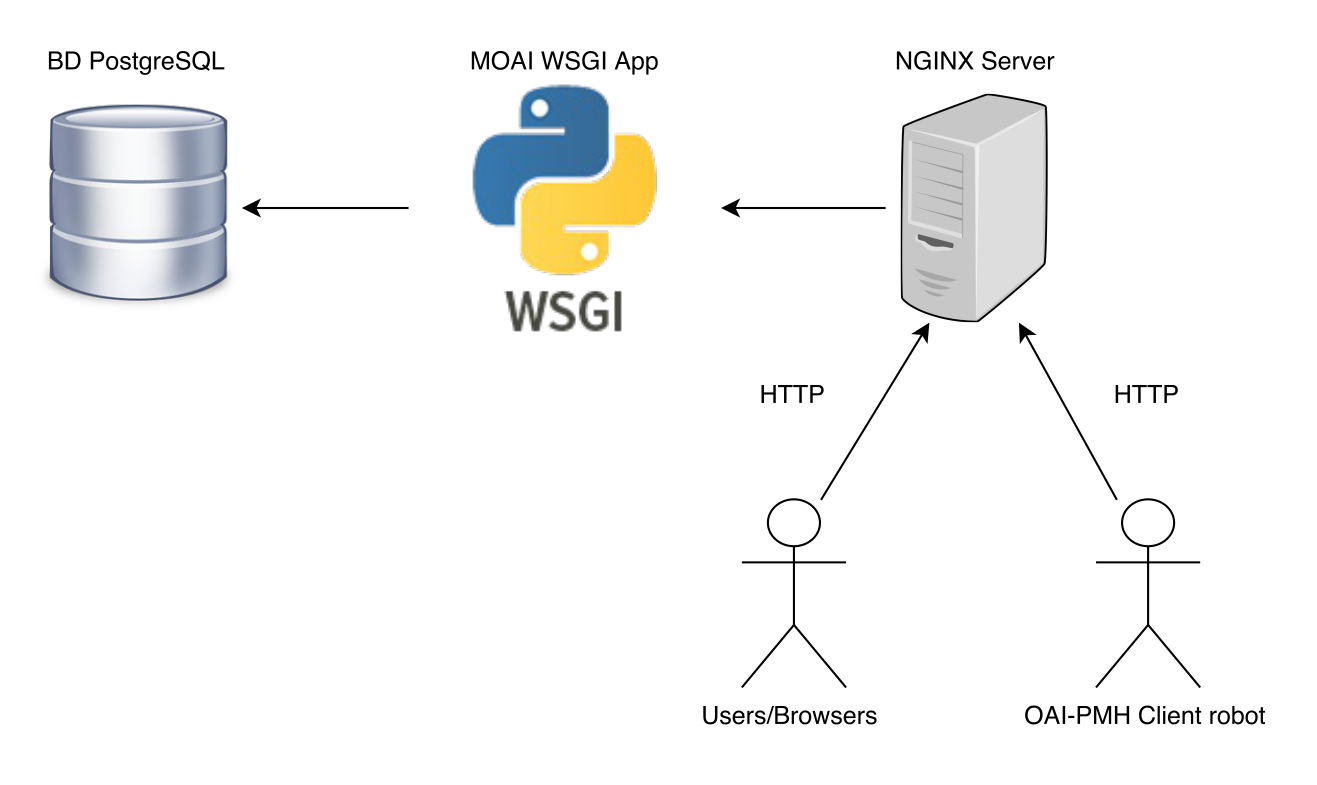
\includegraphics[scale=0.5]{fig/architecture/oai_achitecture}
	\caption{Arquitectura del servidor \acrshort{oaipmh}}
	\label{fig:oai_architecture}
\end{figure}

MOAI es una aplicación dividida en capas, para este proyecto las capas que se han utilizado son las siguientes:

\begin{figure}[!htbp]
	\centering
	\includegraphics[scale=0.5]{fig/architecture/moai_layers}
	\caption{Capas de MOAI}
	\label{fig:moai_layers}
\end{figure}

\begin{itemize}
	\item {Capa de \acrshort{wsgi}:} Capa que implementa la interfaz \acrshort{wsgi} para la redirección del tráfico.
	\item {Capa servidora:} Capa que gestiona los permisos de descargas de los recursos y parsea las \acrshortpl{url}.
	\item {Capa \acrshort{oai}:} Capa que implementa cada uno de los comandos de lo que se compone el protocolo \acrshort{oaipmh}.
	\item {Capa de \acrshort{bd}:} Capa que se conecta a la base de datos y gestiona todas las consultas a ésta.
\end{itemize}

De todas estas capas, ha sido la capa de base de datos la que ha sido modificada para adaptarlo al repositorio de \acrshort{labman}. Por defecto MOAI crea y se conecta a una base de datos SQLite que dispone de tres tablas: Los recursos, los \textit{sets} y por último una tabla de relación de N a M entre éstas dos.

Para adaptar esta capa de datos al repositorio, se ha tenido que definir las dieciocho tablas que almacenan la información sobre las publicaciones y tesis doctorales, así como las tablas de los \textit{logs} de Django, usando SQLAlchemy. Por último se tuvo que definir los métodos \textit{oai\_sets}, \textit{oai\_earliest\_datestamp} y \textit{oai\_query}. Estas funciones son las llamadas que realiza la capa \acrshort{oai} a la capa de \acrshort{bd} para generar el \acrshort{xml} a partir de la información recolectada del repositorio.

\section{Diseño del ``mapeo'' de la Base de datos}

El repositorio de \acrshort{labman} consiste en un conjunto de 120 tablas para almacenar toda la información sobre el grupo de investigación y el propio sistema (véase la figura \ref{fig:labmanmodel}\footnote{Modelo de datos en alta resolución accesible desde \url{https://raw.githubusercontent.com/Alchemy-Meister/PFG/master/fig/dbmodel/high\%20quality/labman\_ud\_models.png}}). Se realizó dicho grafo para tener una visión general de las relaciones internas del modelo relacional.

Sabiendo que dicho servidor OAI iba a publicar solo la información de las publicaciones de los grupos de investigación, se pudo simplificar el modelo relacional completo y a veces incomprensible, debido a el solapamiento de las lineas que simbolizan relaciones, por uno simplificado y dedicado a las publicaciones (véase la figura \ref{fig:publicationsmodel}\footnote{Modelo de datos en alta resolución accesible desde \url{https://raw.githubusercontent.com/Alchemy-Meister/PFG/master/fig/dbmodel/high\%20quality/publications.png}}), lo cual simplificó la tarea del ``mapeo'', dado que la mayoría de la información podía adquirirse desde dicho grafo a excepción de las relaciones externas a las publicaciones, como pueden ser las entidades \textit{Person}, \textit{Tags} y \textit{Languages}. Para visualizar los atributos de éstas últimas se tuvo que seguir haciendo uso del diagrama completo.

\begin{figure}[!htbp]
	\centering
	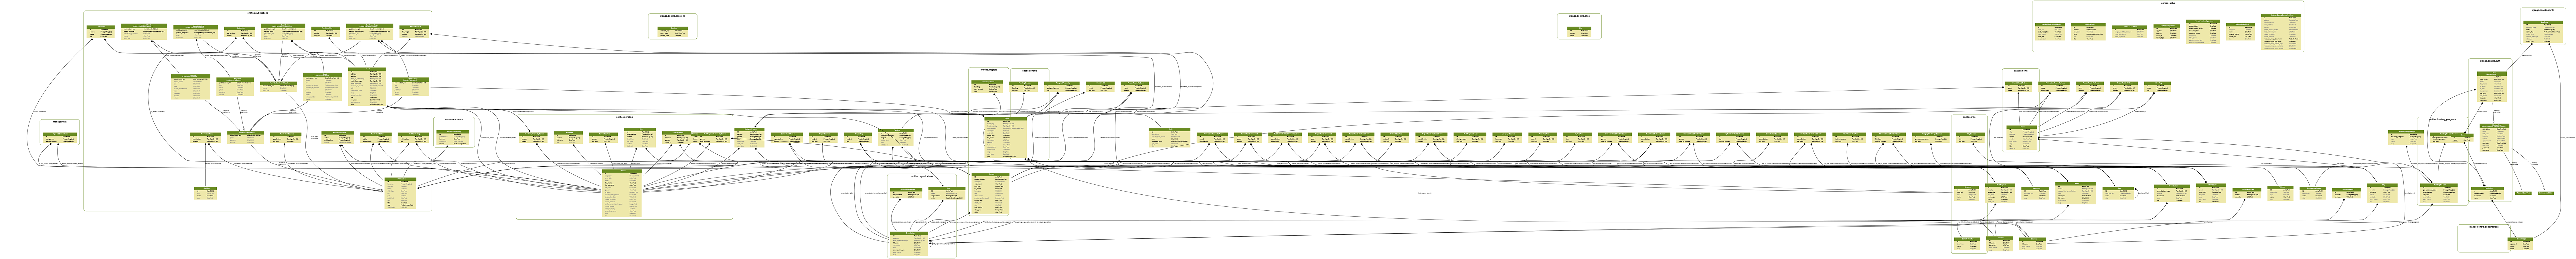
\includegraphics[angle=90, scale=0.072]{fig/dbmodel/labman_model}
	\caption{Modelo de datos relacional completo de \acrshort{labman}}
	\label{fig:labmanmodel}
\end{figure}

Para el desarrollo del servidor se hizo uso de la documentación que proveía la aplicación MOAI para la modificación de la capa de datos. En ésta se detallan los campos de la especificación de \acrshort{dc} que se podían utilizar para el procesado de información y la generación final del \acrshort{xml}. Estos campos y su definición correspondiente son las siguientes:

\begin{itemize}
	\item \textbf{title:} El nombre dado al recursos y por el que es formalmente conocido.
	\item \textbf{creator:} La entidad primaria responsable de la creación del recurso.
	\item \textbf{subject:} El tema que trata el recurso.
	\item \textbf{description:} Documento que puede incluir el resumen o la tabla de contenidos del recurso pero no estar limitado a ellos.
	\item \textbf{publisher:} La entidad responsable de hacer que el recurso este disponible.
	\item \textbf{contributor:} Entidad responsable de hacer contribuciones al recurso.
	\item \textbf{type:} Naturaleza o género del recurso.
	\item \textbf{format:} El formato del fichero o medio físico del documento.
	\item \textbf{identifier:} Una referencia ambigua al recurso.
	\item \textbf{source:} Recursos relacionado que derivan del recurso en cuestión.
	\item \textbf{language:} El lenguaje del recurso.
	\item \textbf{date:} Punto temporal que se asocia con un evento del ciclo de vida del recurso.
	\item \textbf{relation:} Un recurso relacionado.
	\item \textbf{coverage:} La jurisdicción bajo la que un recurso es relevante.
	\item \textbf{rights:} Los derechos de propiedad intelectual a los que se ve asociado el recurso.
\end{itemize}

Esta lista de términos junto con sus definiciones fue necesaria para buscar los campos en la \acrshort{bd} que hacían referencia a estos términos.

Debido al diseño del modelo se descubrió que los tipos de publicaciones, siendo estos actas, ponencias, revistas, artículos de revistas, publicaciones, artículos de publicaciones, libros y secciones de libros, tenían elementos relacionados entre sí. Sin embargo las tesis doctorales estaban formadas por campos completamente independientes por los que se tuvo que realizar un estudio de que elementos de la lista anterior de términos \acrshort{dc} se iban a extraer de la base de datos para las publicaciones y las tesis doctorales por separado quedado el ``mapeo'' resultante tal y como se explica en las subsecciones siguientes.

\subsection{``Mapeo'' de publicaciones}
En la siguiente lista pueden visualizar la relación entre los elementos \acrshort{dc} y las columnas de las tablas referente a las publicaciones con las que se realiza el ``mapeo''.

\begin{itemize}
	\item \textbf{title:} entities.publication.publication.title.
	\item \textbf{creator:} person.full\_name relacionado con entities.publication.publicationauthor.author.
	\item \textbf{subject:} tag.name relacionado con entities.publication.publicationtag.
	\item \textbf{description:} entities.publication.publication.abstract.
	\item \textbf{publisher:} entitites.publication.collectionpublication.publisher.
	\item \textbf{type:} entities.publication.publication.childtype.
	\item \textbf{format:} Valor estático ``digital''.
	\item \textbf{identifier:} Concatenación de los campos id y slug de entities.publication.publication
	\item \textbf{language:} language.language\_tag relacionado con entities.publication.publication.language, valor estático ``en'' en caso de null.
	\item \textbf{date:} entities.publication.publication.
\end{itemize}

\begin{figure}[!htbp]
	\centering
	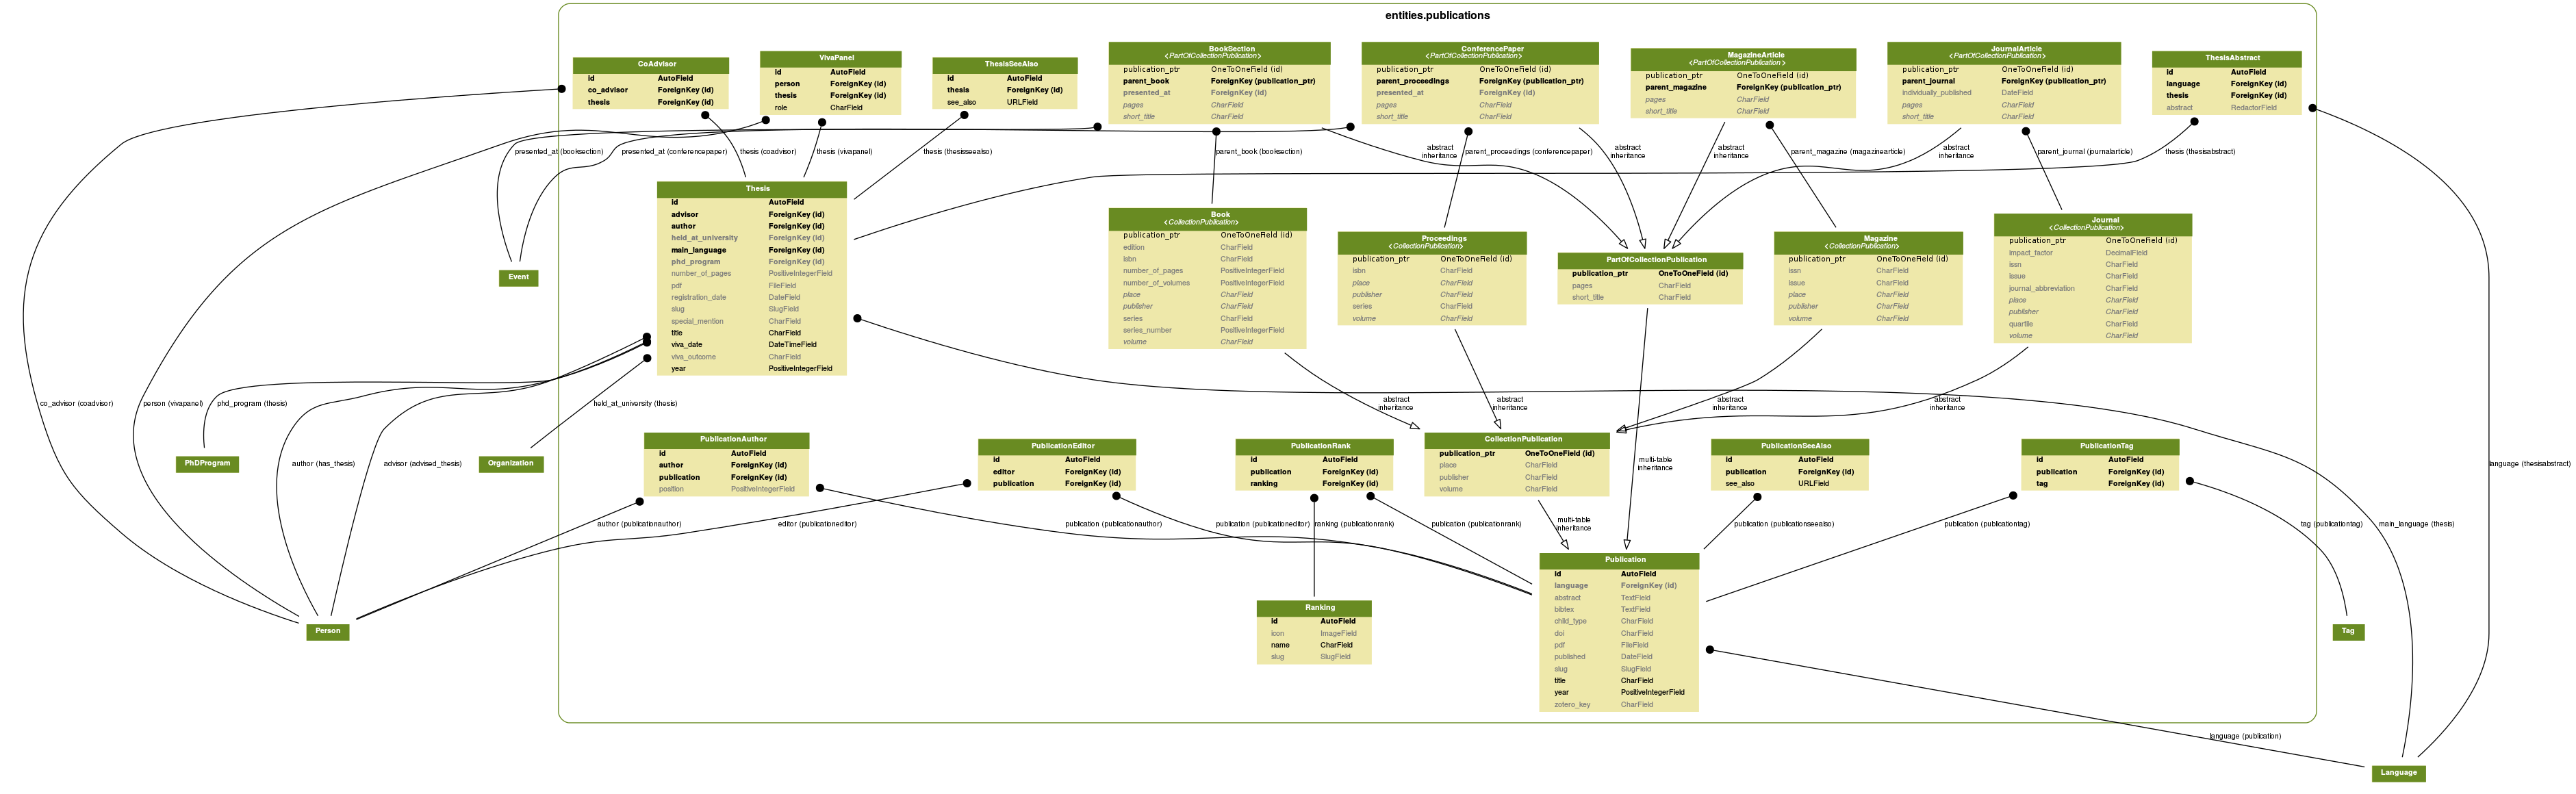
\includegraphics[angle=90, scale=0.17]{fig/dbmodel/publications}
	\caption{Modelo de datos relacional de las publicaciones}
	\label{fig:publicationsmodel}
\end{figure}

\subsection{``Mapeo'' de tesis doctorales}

En la siguiente lista se pueden visualizar la relación entre los elementos \acrshort{dc} y las columnas de las tablas referente a las tesis doctorales con las que se realiza el ``mapeo''.

\begin{itemize}
	\item \textbf{title:} entities.publication.thesis.title.
	\item \textbf{creator:} person.full\_name relacionado con entities.publication.thesis.author.
	\item \textbf{description:} publication.thesisabstract.abstract relacionado con entities.publication.thesis. id.
	\item \textbf{type:} Valor estático ``doctoral dissertation''.
	\item \textbf{format:} Valor estático ``digital''.
	\item \textbf{identifier:} Concatenación de los campos id y slug de entities.publication.publication.
	\item \textbf{language:} language.language\_tag relacionado con entities.publication.thesis.main\_ language.
	\item \textbf{date:} entities.publication.thesis.registration\_date, no mostrar en caso de null.
\end{itemize}

\section{Diseño de la aplicación web}

El cliente web es una extensión del sistema \acrshort{labman}. La aportación realizada en este proyecto pretende mejorar su funcionalidad mediante la implementación de un buscador avanzado de publicaciones y proyectos para facilitar el acceso a la información deseada.

El cliente web ha sido diseñado usando los elementos proporcionados por Django para los elementos estáticos, validación de formularios, a demás se ha utilizado jQuery para añadir funcionalidad dinámica, \acrshort{html} para el contenido y por último \acrshort{css} y Bootstrap para el diseño.

Al igual que con el servidor de MOAI, el diseño de la \acrshort{bd} ya venía preestablecido, pero se ha requerido hacer un estudio de las entidades del modelo de datos relacionados con las publicaciones, como ya se ha podido ver en la figura \ref{fig:publicationsmodel}, así como el modelo de proyectos (véase la figura \ref{fig:projectsmodel}\footnote{Modelo de datos en alta resolución accesible desde \url{https://raw.githubusercontent.com/Alchemy-Meister/PFG/master/fig/dbmodel/high\%20quality/projects.png}}), para realizar el filtrado de la información a partir de un subconjunto de sus facetas.

Django se basa en la arquitectura \acrshort{mvc} (véase la figura \ref{fig:mvc}) en la que el usuario interactua con el controlador actualizando la vista para introducir los valores en las facetas sobre las que desea filtrar la información y al realizar la búsqueda, el controlador consulta el modelo, obtiene la información requerida por el usuario y actualiza la vista.

\begin{figure}[!htbp]
	\centering
	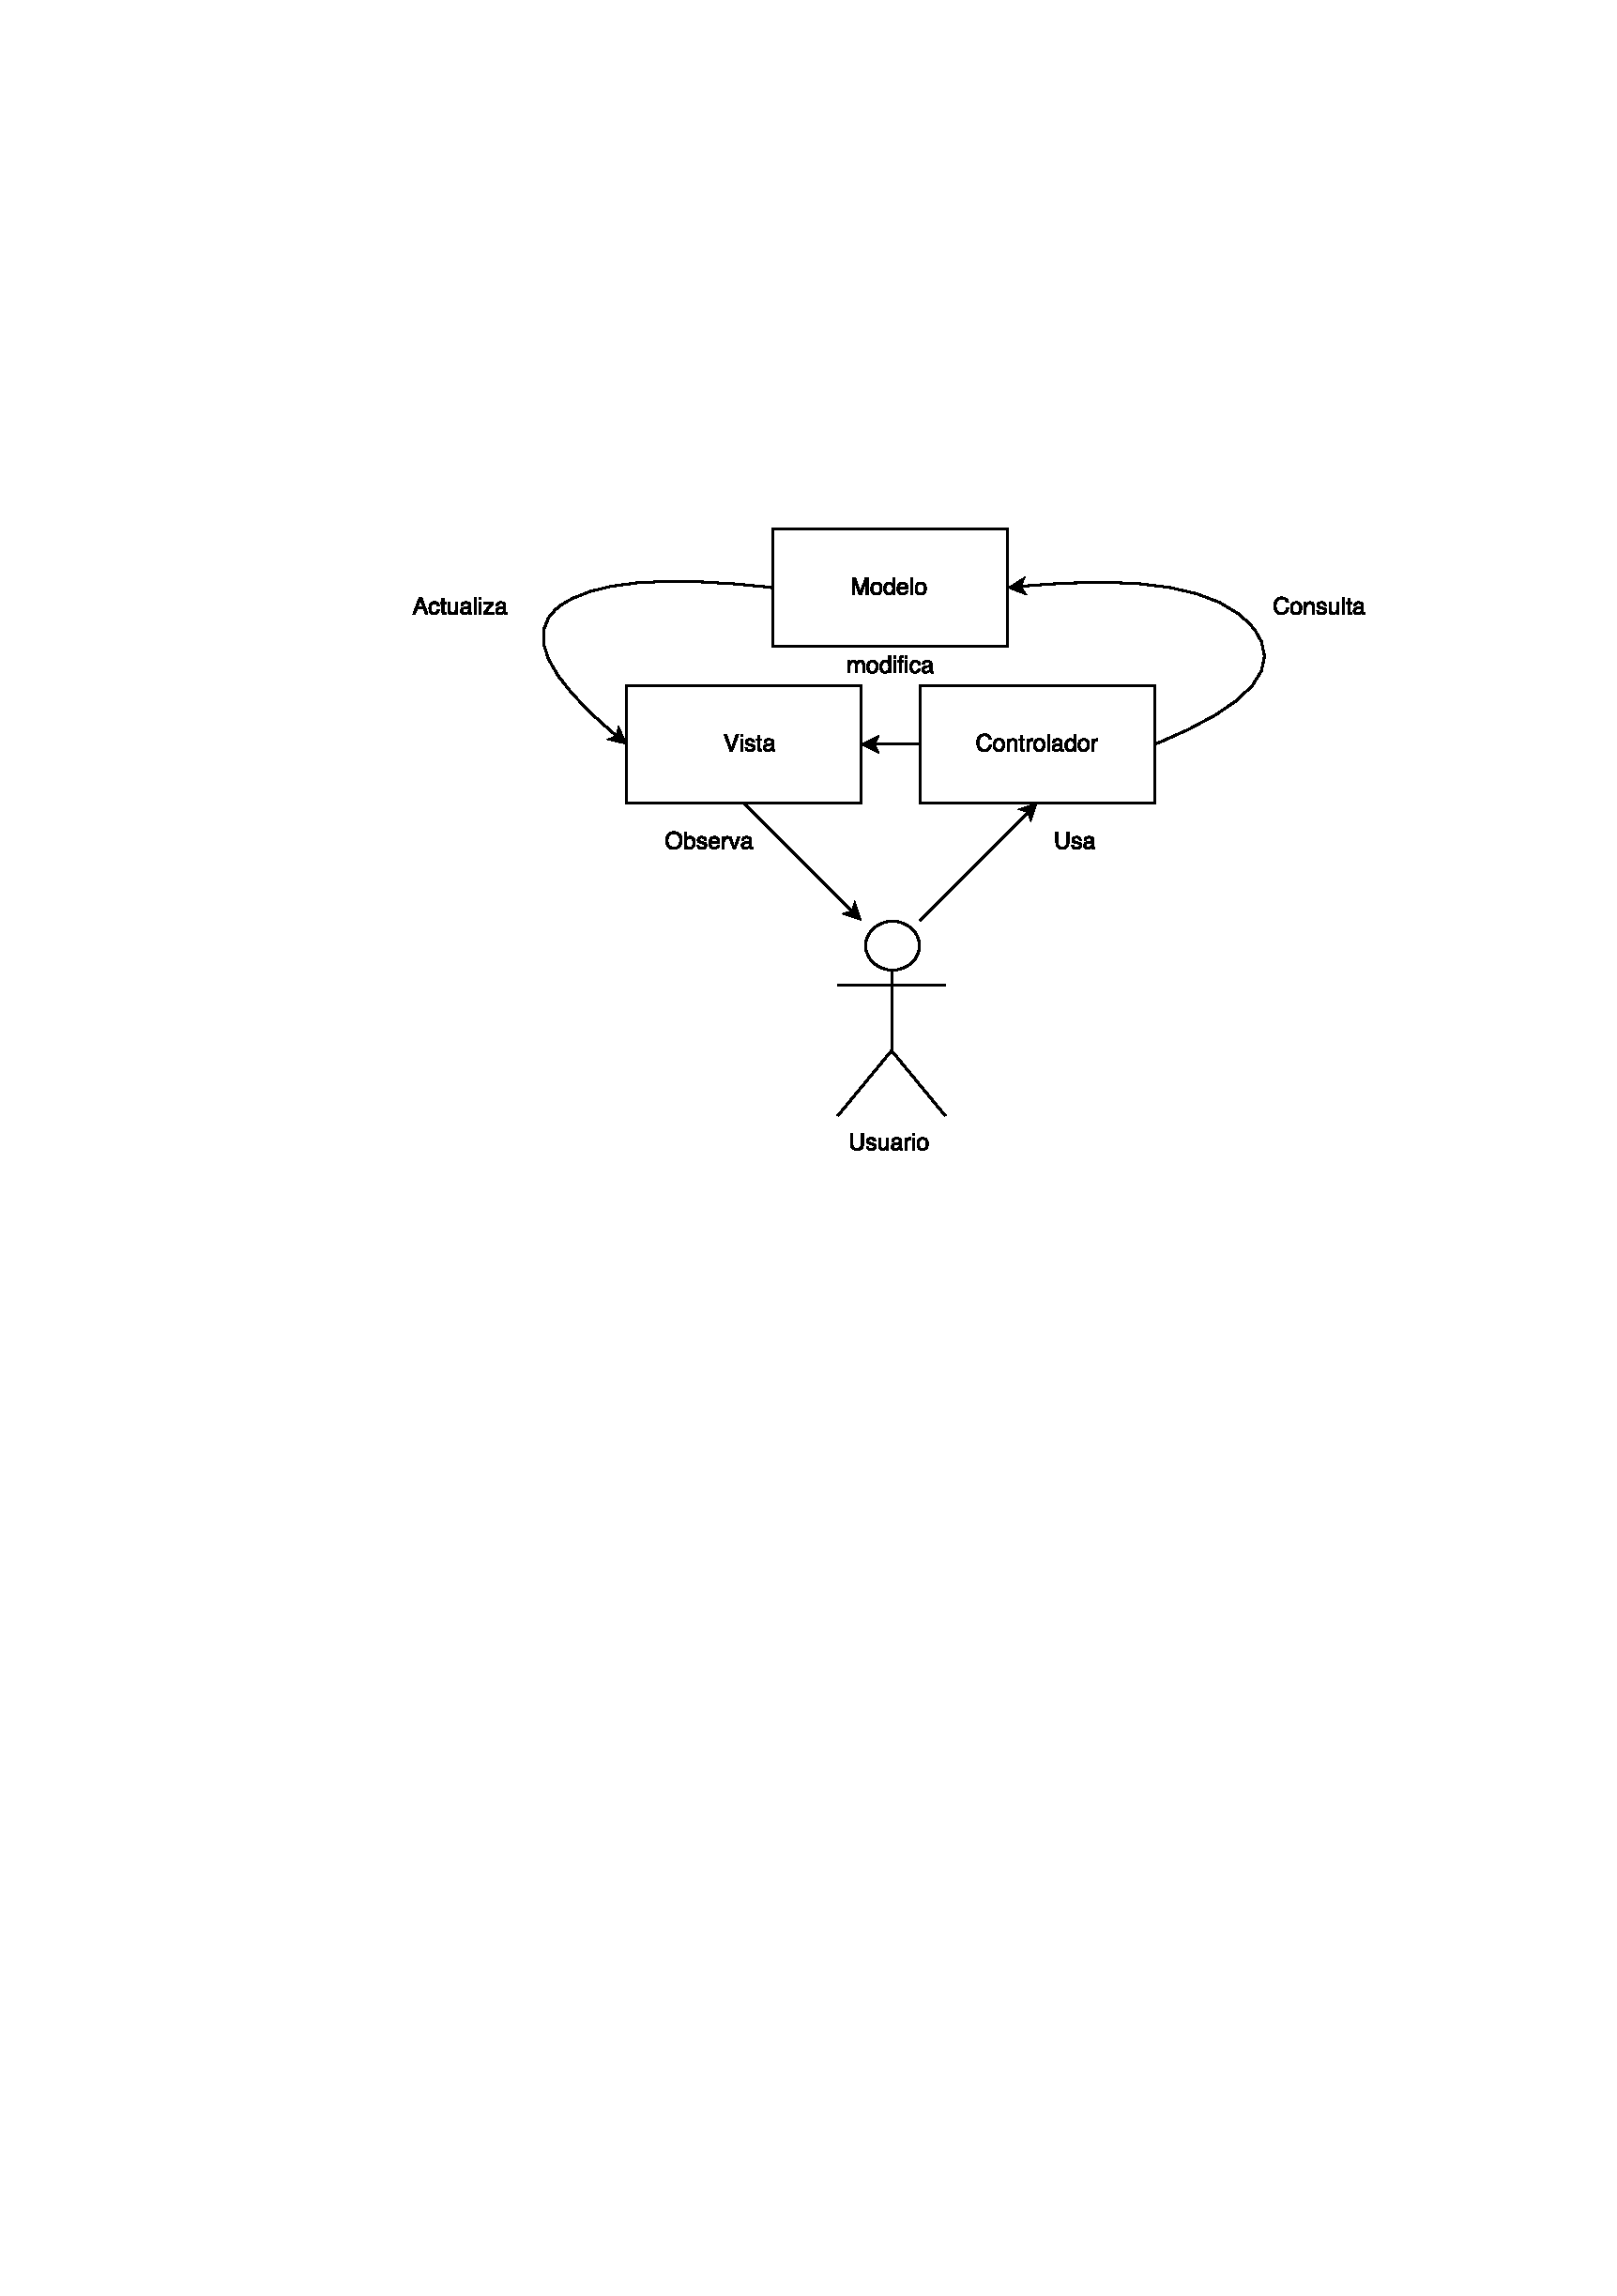
\includegraphics[scale=0.6]{fig/mvc}
	\caption{Arquitectura \acrshort{mvc} del cliente web}
	\label{fig:mvc}
\end{figure}

\begin{figure}[!htbp]
	\centering
	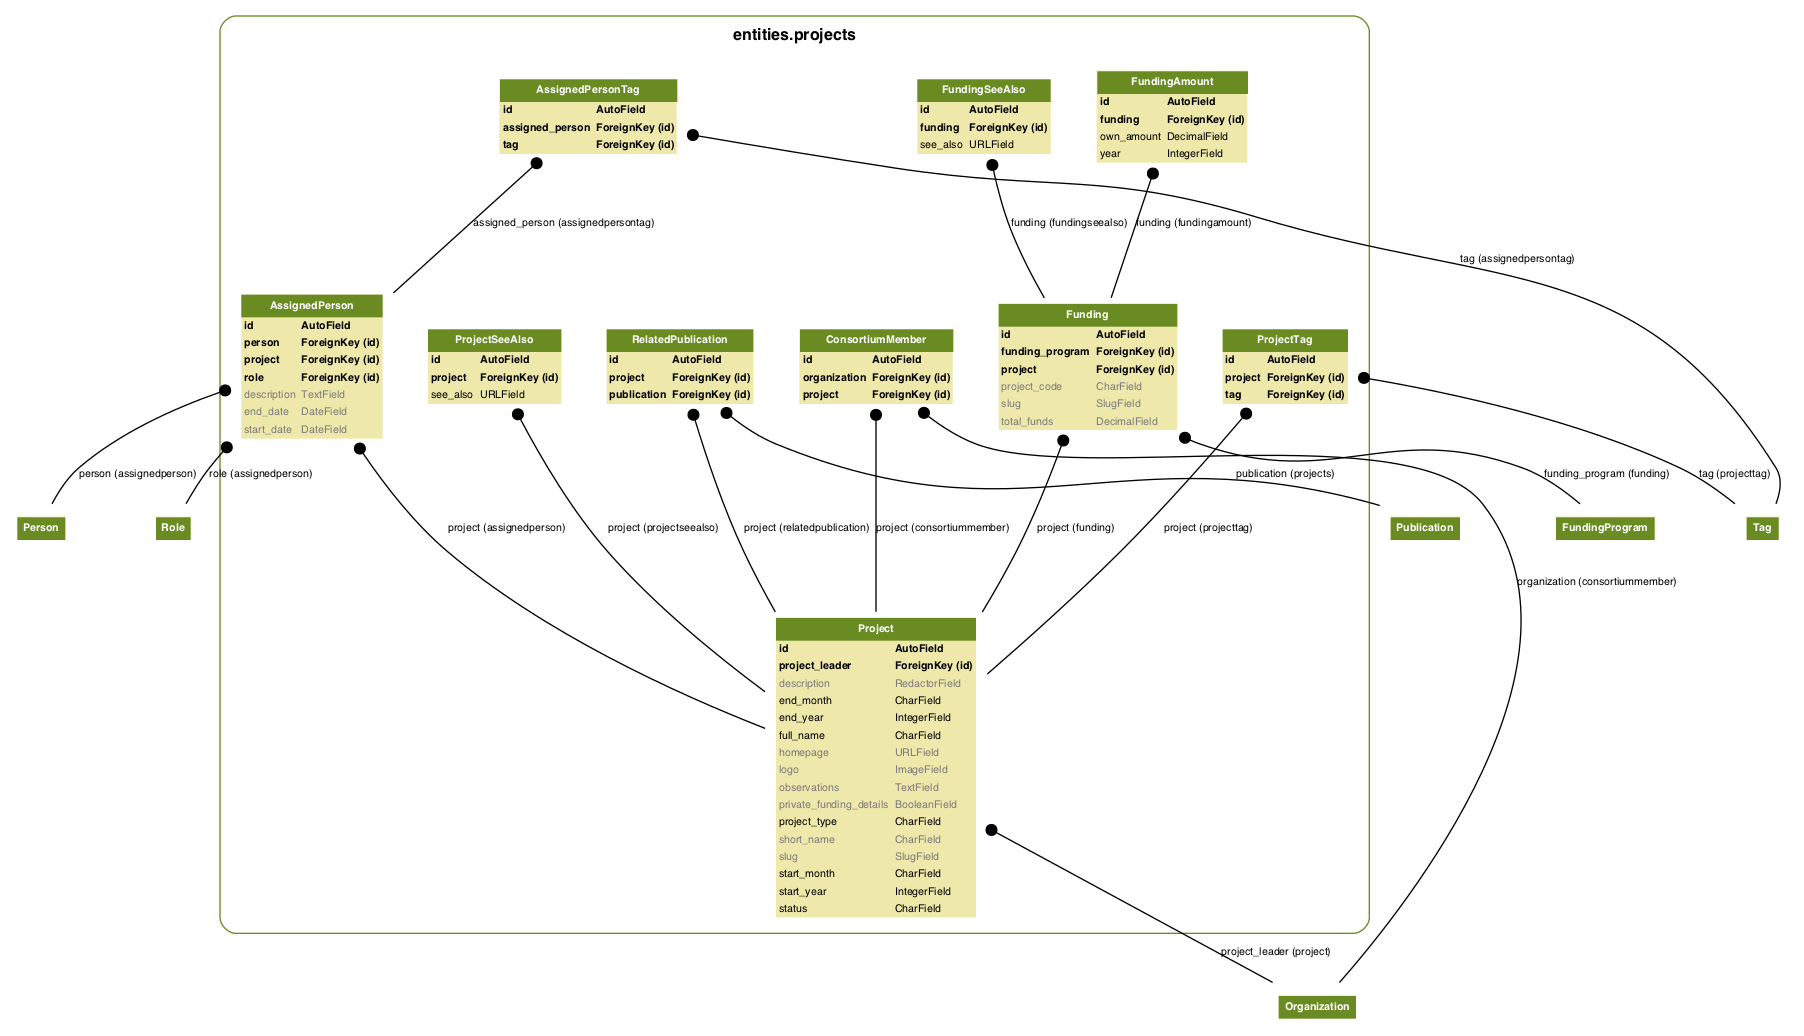
\includegraphics[angle=90, scale=0.35]{fig/dbmodel/projects}
	\caption{Modelo de datos relacional de las proyectos}
	\label{fig:projectsmodel}
\end{figure}

Al extender un proyecto en producción como lo es \acrshort{labman} el diseño del modelo de datos ha sido nulo, dado que ya había sido todo implementado por su creador Oscar Peña. Sin embargo, ha sido necesario hacer uso de la implementación para poder mejorar la usabilidad del portal web e implementar el buscador avanzado.

A partir del diseño de la interfaz de usuario (Vista) se recogen los valores de las facetas por las que se quiere filtrar los recursos sobre los proyectos o publicaciones a través de peticiones POST. Es entonces cuando el controlador verifica la validez del formulario y realiza las consultas a la \acrshort{bd} (Modelo) a través del \acrshort{orm} de Django. Mediante estas consultas se obtienen los datos requeridos por el usuario, así como valores extra que requiere la vista para actualizarse correctamente. El controlador devuelve estos valores a la vista para que el usuario pueda visualizar la vista. Este proceso se detalla mejor en la figura \ref{fig:project_flow_diagram} que representa un diagrama de flujo del proceso simplificado del filtrado de los proyectos que se produce en el controlador.

\begin{figure}[!htbp]
	\centering
	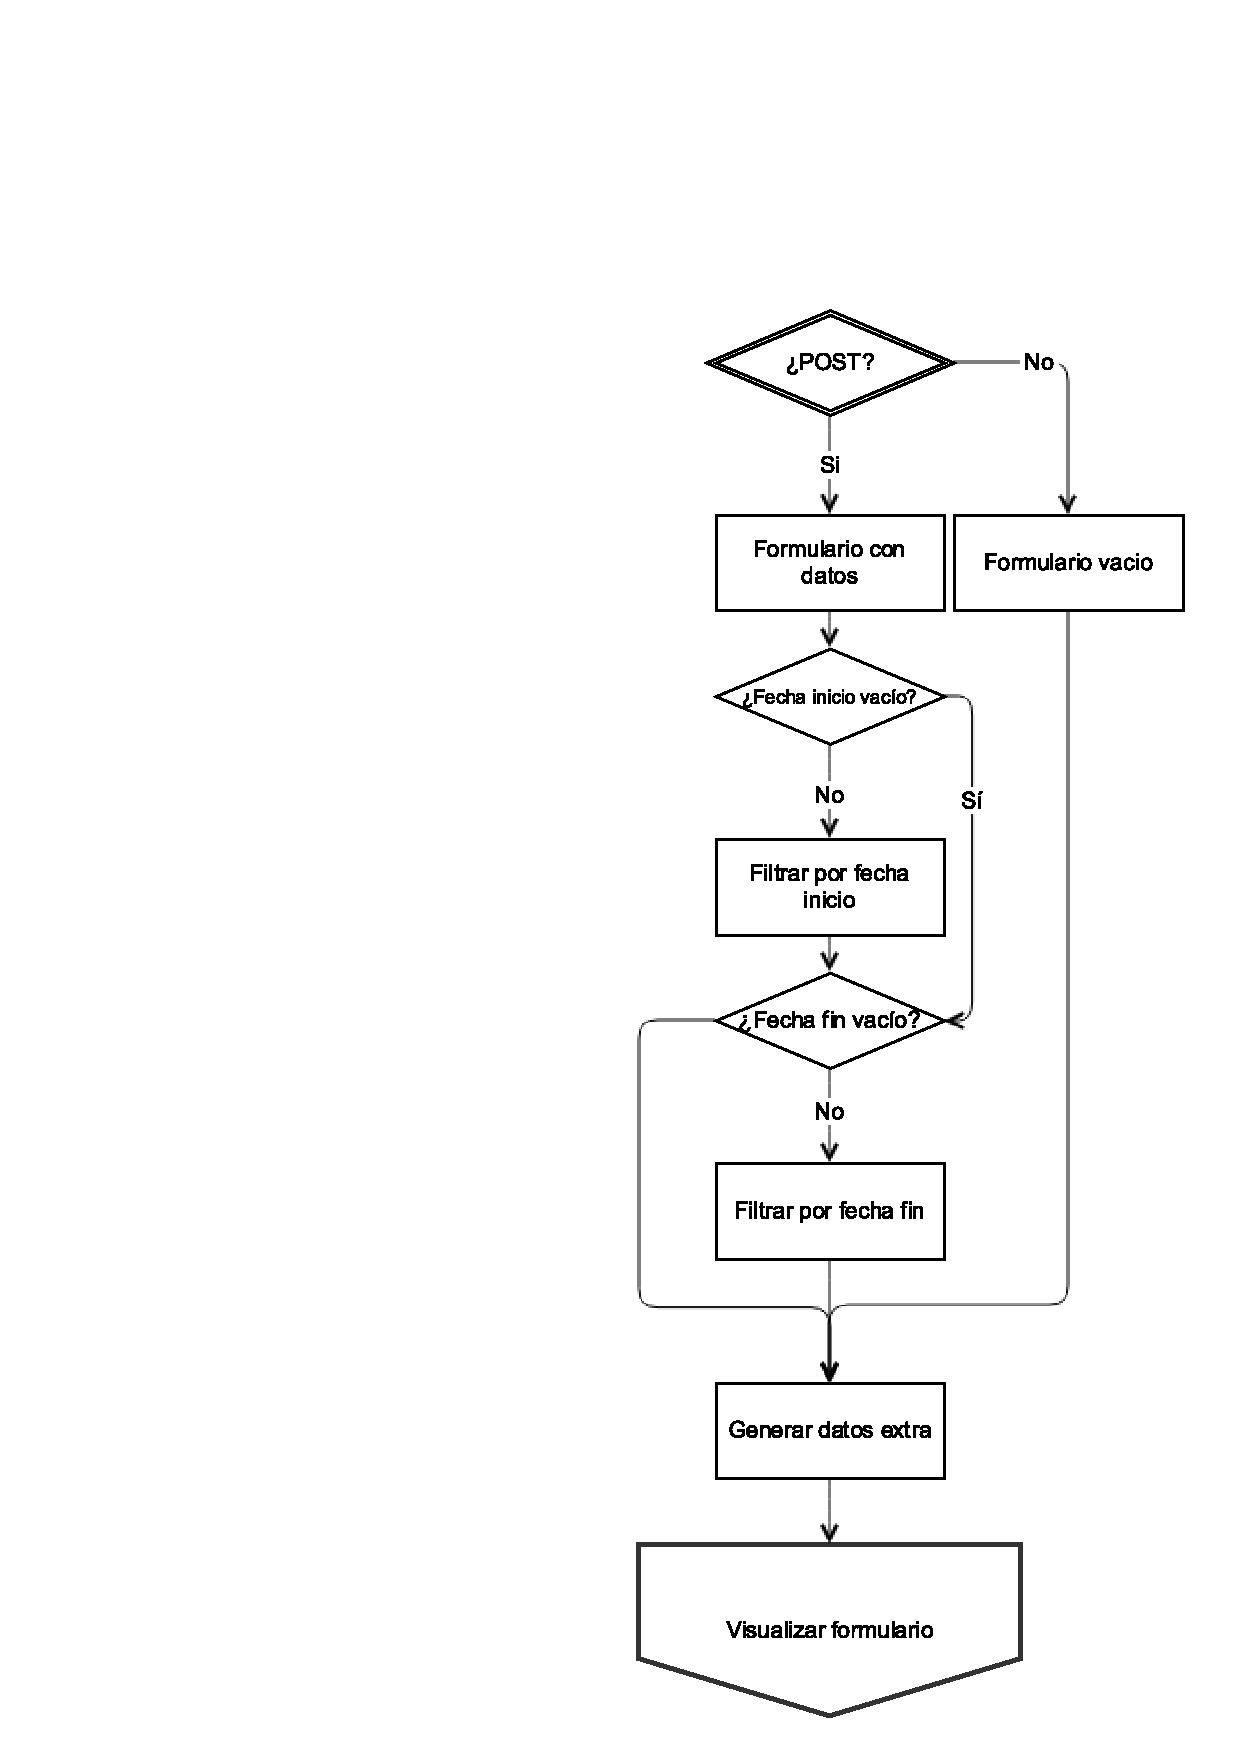
\includegraphics[scale=0.6]{fig/flow}
	\caption{Diagrama de flujo simplificado del proceso de filtrado de proyectos}
	\label{fig:project_flow_diagram}
\end{figure}